\chapter*{Simple examples about latex code}
\label{cha:samples}

\section{reference samples}
\label{sec:refSamples}

\begin{figure}[!h]
	\centering
	%or \columnwidth
	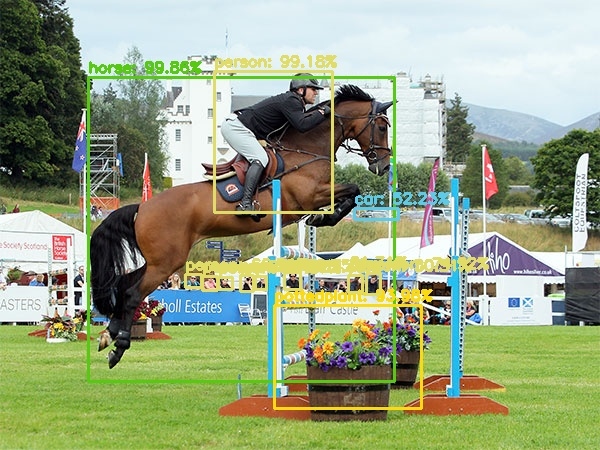
\includegraphics[width=0.3\linewidth]{images/ex1_yolo.jpg} %.jpg is useless
	\caption{Object detection applied on a sample image.}
	\label{fig:sampleYolo}
\end{figure}

\begin{table}[h]
	\centering
	\begin{tabular}{ll|l|ll}
		\cline{1-4}
		\multicolumn{1}{|l|}{c} & i & a & \multicolumn{1}{l|}{o} &                        \\ \hline
		\multicolumn{1}{l|}{}   & c & o & \multicolumn{1}{l|}{m} & \multicolumn{1}{l|}{e} \\ \cline{2-5} 
		\multicolumn{1}{l|}{}   & v & a &                        &                        \\ \cline{2-3}
		&   & ? &                        &                        \\ \cline{3-3}
	\end{tabular}
	\caption{Example table.}
	\label{tab:sampleTable}
\end{table}

Try to cite different elements\footnote{Not only reference but also footnote ;)}:
\begin{itemize}
	\item images show at: \Cref{fig:peoplePair}\\
		  more complex images can be found at: \href{https://tex.stackexchange.com/questions/37581/latex-figures-side-by-side}{side by side images}
	\item look at \Cref{tab:sampleTable}\\
	it can be generatedonline at this \href{https://www.tablesgenerator.com/}{online editor}.
	\item the sample chapter can be found at: \Cref{cha:samples}
	\item precisely at \Cref{sec:refSamples}
	\item yolov3 \cite{yoloV3}
\end{itemize}

